%%-------------Summary of the chapter -------------
An energy-harvesting intermittent node frequently switches between off and on, charging energy and operating. We can characterize, from a time perspective, this charge-discharge cycle (or power cycle) using the following notation: ($t_\text{on}$, $t_\text{p}$), where $t_\text{on}$ refers to a node's uptime interval, and $t_\text{p} \coloneqq t_\text{on} + t_\text{off}$, where $t_\text{off}$ refers to a node's charging time interval.

The \fullsys (\sys) is the abstraction of a group of intermittent senor nodes seeking to mimic the continuous sensing availability characteristic of a battery-powered sensor. 
%
The design of \sys needs to consider three main aspects: (i) how the nodes' awake time is distributed, (ii) the effect of the environment on \sys's availability and what is needed to mitigate it, and (iii) the consequence of approaching continuous sensing availability in a discrete fashion.  
%
% Unfortunately, the dependency of \sys's nodes on ambient energy and the effect of incoming events on their power cycles render out the option of simply grouping $N$ nodes and hoping that their collective availability would be ($N\times t_\text{on}, t_\text{p}$).
% Therefore, the rest of this section studies the \sys's availability, how it evolves when additional nodes are added, the effect of the environment and what is needed to mitigate it, and the consequence of approaching continuous sensing availability in a discrete fashion. 


% define CIS
% The \fullsys (\sys) is the abstraction of a group of battery-less intermittent senor nodes seeking to mimic the continuous availability characteristic of a battery-powered sensor. 
% %
% The first question to ask when designing a \sys is what is the minimum number of intermittent sensors needed to approach required collective availability?
% %
% Further, if the power cycles of the nodes are synchronized (e.g., on an incoming event), then adding more nodes has no value as their uptimes will not spread in time to increase the collective availability. Will that happen? If yes, how to prevented?
% %
% Finally, what is the effect of approaching continuous availability in a discrete fashion on sensing? The rest of this section is devoted to answer the above questions.

% % analyze energy consumption (event-based vs polling sensing)
% To this end, we will first analyze the energy-consumption life cycle of an intermittently-powered node, as well as the joined availability of multiple nodes. 
% % favorable energy condition problem
% Then we will point out a practical aspect that is often overlooked; when intermittent nodes operate in favorable ambient conditions, their uncorrelated behavior changes due to the extra energy leading to synchronized patterns that need to be scrambled by introducing artificial, controlled randomization.
%%  ------------- ------------- -------------
%
\begin{figure}[t]
		\centering
		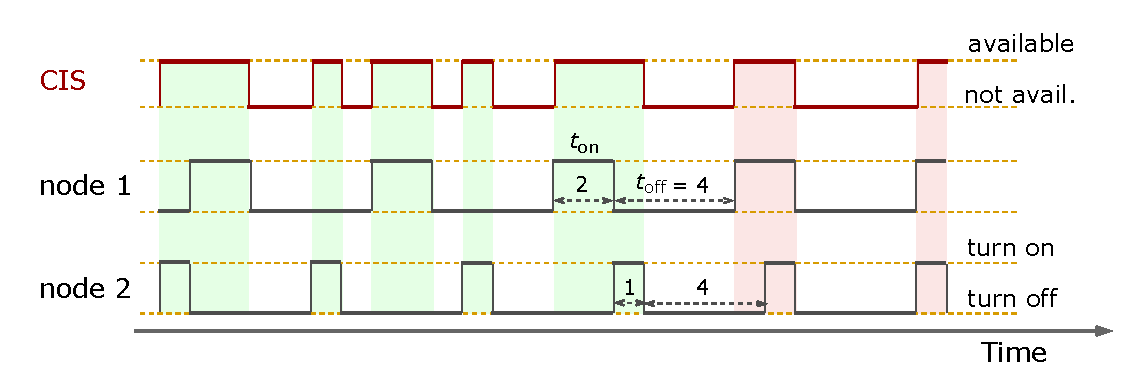
\includegraphics[width=\columnwidth]{figures/cisOntime}
		\caption{A \fullsys's availability is the emerging collective on-time of its intermittent nodes' on-times. The difference between the power cycles leads to a constant relative shift between the nodes duty cycles. This, in turn, causes their on-times to be uniformly distributed on the overall power cycle. The red bars indicate a minimum \sys time span---\sys's nodes are overlapping---whereas the green bars show the maximum time span of the \sys.}
		\label{fig:cisOntime}
\end{figure} 
%
\subsection{Sensing}

The ability of \sys to sense depends on the availability of its intermittent nodes and on the characteristics of the event of interest. 

\subsubsection{Coalesced availability}
\label{subSec:availability}
%
The \sys's on-time (availability) is the projection of its underlying intermittent nodes' on-times on the time axis. Thus, it can anywhere between a minimum (when all nodes' on-times cluster together) and a maximum (when the overlapping between on-times cannot be any smaller), depending on the nodes spreading strategy being employed.
%
In general, we can imagine two broad spreading strategies:

\noindent \textbf{Explicit on-time division strategy}: 
% ToDo [Discuss with Koen] maybe because of this section, one of the reviewers
% stated that he is not sure if the overhead is justifiable 
Ultra-low-power timers have enabled intermittent nodes to time their $t_\text{on}$ and $t_\text{off}$~\cite{hester2017timely}.
%
Recent advancements in passive light (or RF) communication have enabled nodes to efficiently backscatter messages on top of ambient light (or RF signals)~\cite{LuzLink,liu2013ambient}. 
% (or RF) communication has the potential to enable intermittent sensors to exchange messages with very minimal energy consumption (for example, nodes embedded in wallpaper, see Figure~\ref{fig:smart_fabric}, can backscatter on top of room light to communicate)~\cite{LuzLink}.
% Similar breakthroughs in passive communication have enabled ultra-low-power message exchange between battery-less nodes~\cite{li2015retro}. 
%
A \sys can build on top of these advancements to apply a time-division multiplexing strategy to minimize  on-times overlapping.
%
For example, a node calculates its average on-time $\overline{t_\text{on}}$ and off-time $\overline{t_\text{off}}$ for $N$ power cycles. Then it measures the time difference between its power-up and the intended transmitting time $\Delta\,t$. Subsequently, it encodes the information $({\overline{t_\text{off}}, \overline{t_\text{on}}, \Delta\,t})$ in a message and broadcasts it. When a node receives this message it will have full knowledge about the transmitting node's power cycle. It can then alter its power cycle, relative to the transmitting nodes cycle, by either increasing (or decreasing) its power consumption to shorten (or lengthen) its on-time and subsequently shifting its power cycle to a different time slot. 
% 
% Obviously, the effectiveness of this approach hinges on the stability of individual nodes' power cycles. 
% Figure~\ref{fig:power_cycles} shows that the power cycles of solar powered nodes are more stable than RF counterparts~\footnote{Make sure to observe the difference of the length of the power cycles of solar and RF powered nodes.}. Therefore, this approach 
% A relatively stable power cycles are observed specially when the nodes harvest solar power, see Figure~\ref{fig:power_cycles}.

With such explicit on-times control strategy, a \sys of $N$ nodes with average $\overline{t_\text{on}}$ and off-time $\overline{t_\text{off}}$ will have an average availability of $N\times \overline{t_\text{on}}$ (or 100\% if the total length of the on-times exceeds the nodes longest power cycle).
%
\begin{figure}
		\centering
		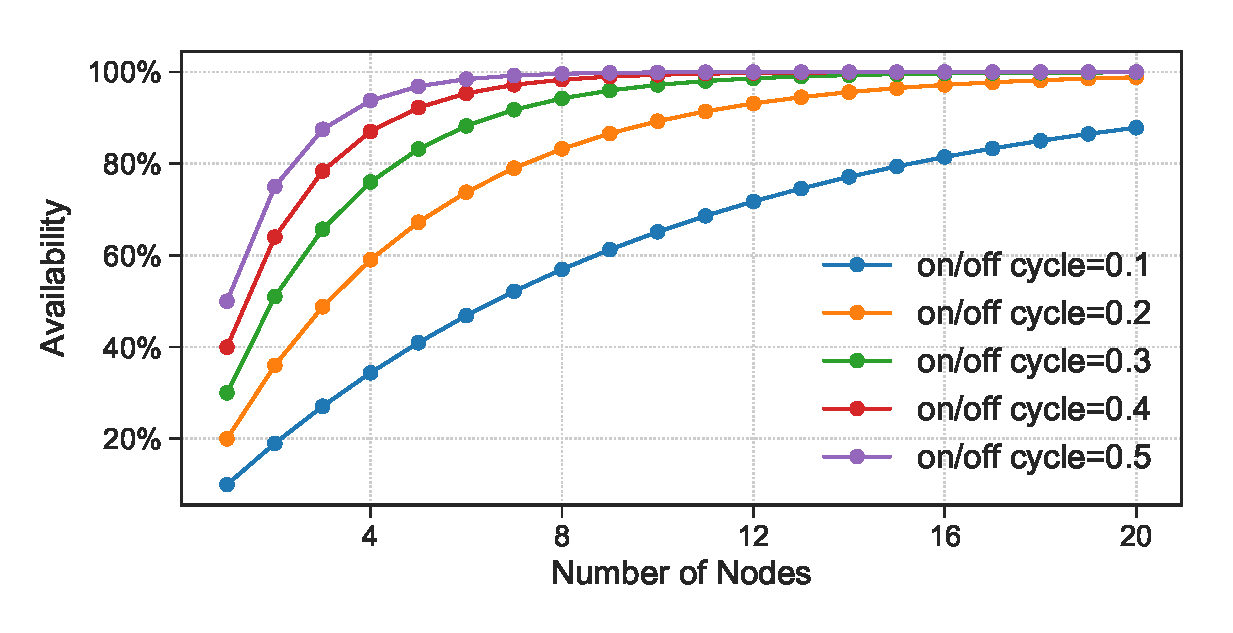
\includegraphics[width=\columnwidth]{figures/cisModel}
		\caption{\fullsys availability percentage for a different number of nodes and different duty cycles. The nodes are uniformly distributed and the \sys on-time evolves, when adding new nodes, according to the equation~\ref{eq:cisModel}.}
		\label{fig:cisModel}
\end{figure} 

\noindent\textbf{Implicit on-time division strategy}: 
% The key to success is to exploit the properties (i.e.\ randomness) of the ambient energy source to arrive at a uniform spreading of the awake times of the individual senor nodes to achieve the maximum coalesced availability. 
With no information being exchanged between intermittent nodes, the best \sys can do is to uniformly distribute its node's on-times and maintaining this distribution over time. 
The key observation to approach uniform distribution is to ensure that the node's power cycles are randomized.
% The key observation to distribute nodes' on-times uniformly is to ensure that their power cycles are randomized.

\noindent\textit{Idealized power cycles.}
Let us assume that we have two nodes with ideal power cycles characterized by ($t_\text{on}$, $t_\text{p}$), and they have the same initial conditions. The collective on-time of these two nodes will still be $t_\text{on}$ as they are in perfect synchronization (the two nodes wake up and power down together). 
% 
To desynchronize their awake times a node should alter its power consumption, by sleeping for example, to shift its on-time to a different time slot. 
% awake for a certain interval extends the node's on-time by $\Delta t$. 
% in low-power mode, forcing it to consume less energy to prolong its on-time to be  ($t_\text{on} +\Delta t$).
% Doing so once shifts the node awake time relative to the position of the other node uptime by $\Delta t$. 
% However, since we do not assume communication
If we relax our assumptions, however, saying that the initial conditions are unknown, then shifting the on-time a constant number of times may cause the initially desynchronized nodes to be synchronized, reducing the \sys's availability instead of extending it.  However, if the node constantly extends its on-time (and subsequently its power cycle), then its on-time will shift over the entire power cycle of the other node, spending 
$\frac{ t_\text{off} }{t_\text{p}}$ and $\frac{ t_\text{on} }{t_\text{p}}$ of the time overlapping with its off-time and on-time, respectively. 
 This behavior is illustrated in Figure~\ref{fig:cisOntime}, where node 1 has a power cycle of (2,6) and node 2 has a (1,5) power cycle.
Following the time axis from the left to the right, we can see that the position of the on-time of node 2 is shifted by 1 unit of time after each power cycle of node 2. This implies that the on-times of the two nodes are $\frac{1}{3}$ of the time cluster together and $\frac{2}{3}$ of the time they are apart. If we extend the previous scenario to three or more nodes then the on-time of the resulting \sys can be described with the following formula,
				
\begin{equation}
	t_\text{on}(N) = t_\text{on}(N-1) + \frac{t_\text{off}(N-1)}{t_\text{off}(N-1)+t_\text{on}(N-1)} \times t_\text{on}(1),
		\label{eq:cisModel}
\end{equation}
where $N \in \mathbb{N}$ and  $t_\text{on}(N)$ is the on-time of a \sys with $N$ intermittent nodes. For the initial case where $N=1$ we define $t_\text{on}(0)\coloneqq 0$ and $t_\text{off}(0) \coloneqq 1$. We further show in Figure~\ref{fig:cisModel} the \sys's availability for different duty cycles and different number of intermittent nodes.
% In addition to characterizing the availability of a \sys, equation~\ref{eq:cisModel} also states that the benefit of adding a node to the \sys is proportional to the \sys's off-time.
% In Figure~\ref{fig:cisModel} \sys availability percentage for different duty cycles and different number of intermittent nodes are shown.
\noindent\textit{Natural power cycles.}
In reality, intermittent nodes power cycles are different, and they are not constant (Figure~\ref{fig:power_cycles}). However, differences between the power cycles and their embedded randomness are sufficient conditions to force their on-times to be in constant shift relative to each other and approach uniform distribution (Figure~\ref{eq:cisModel})
\todo{support this claim using simulation}. 

There is a clear trade-off between the aforementioned methods. While the explicit control method provides fine control over the system 
distribution and therefore requires less number of nodes than the implicit control method, the implicit control method does not depend on the ability to communicate between the nodes and therefore it is simpler and more energy efficient. Since inter-node communication is beyond the capabilities of most of today's intermittent nodes, \textbf{the rest of the paper considers only the implicit approach}.
 
%Although the implicit method is relatively simple to implement and explore, the explicit control method is not a far-fetched idea considering the recent advancements in passive communication and intermittent timing. However, we opt to explore the implicit distribution control method as the hardware used to demonstrate the feasibility of passive light communication and ambient RF backscattering are not open source and re-making it is beyond the scope of this study.

\begin{figure}[t]
		% \begin{subfigure}{.49\columnwidth}
		% 	\centering
		% 	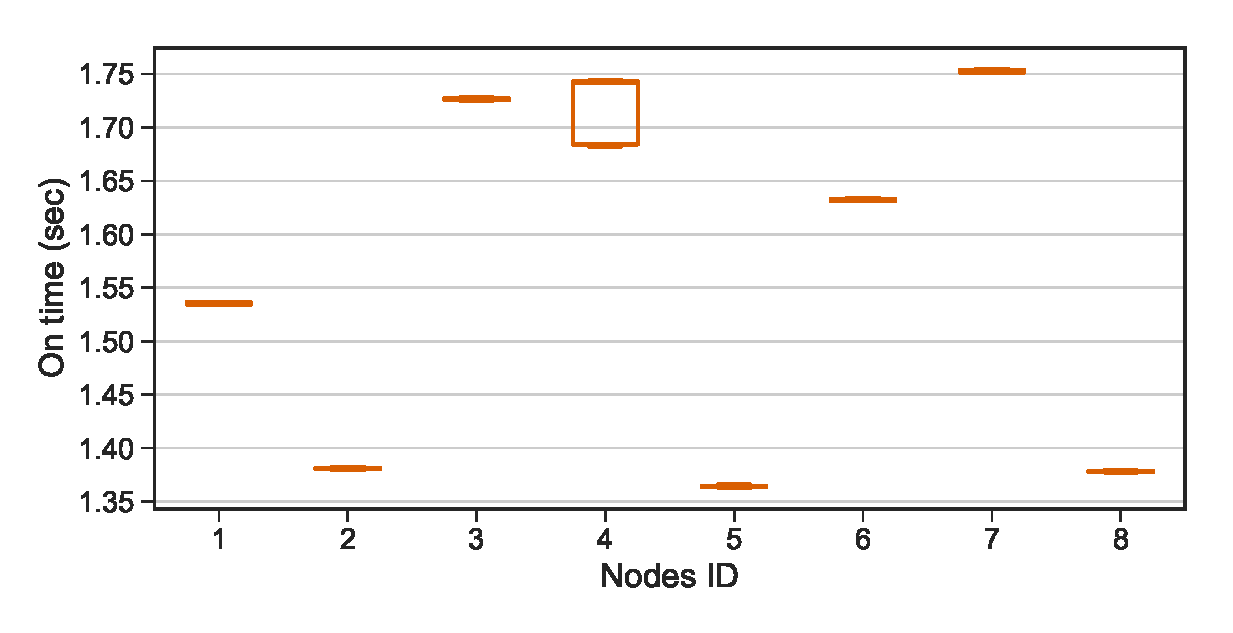
\includegraphics[width=\textwidth]{figures/light_on_time}
		% 	\caption{light}
		% \end{subfigure} \hfill
		% \begin{subfigure}{.49\columnwidth}
		% 	\centering
		% 	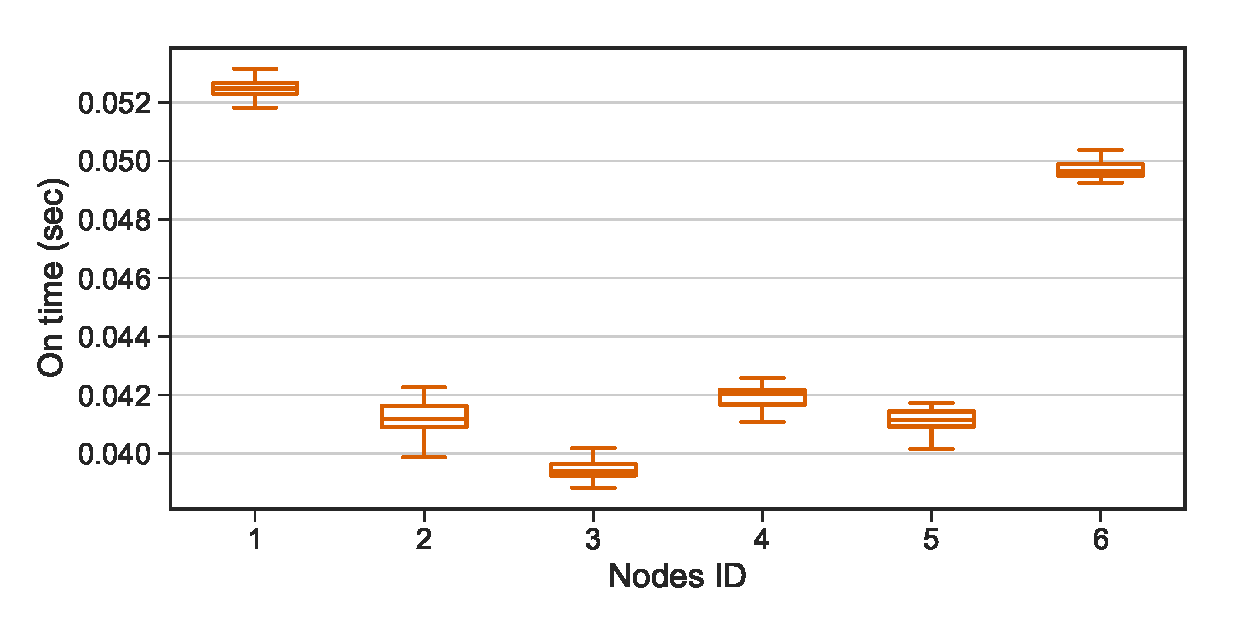
\includegraphics[width=\textwidth]{figures/rf_on_time}
		% 		\caption{RF}
		% \end{subfigure}\hfill
		%
		
		\begin{subfigure}{.49\columnwidth}
			\centering
			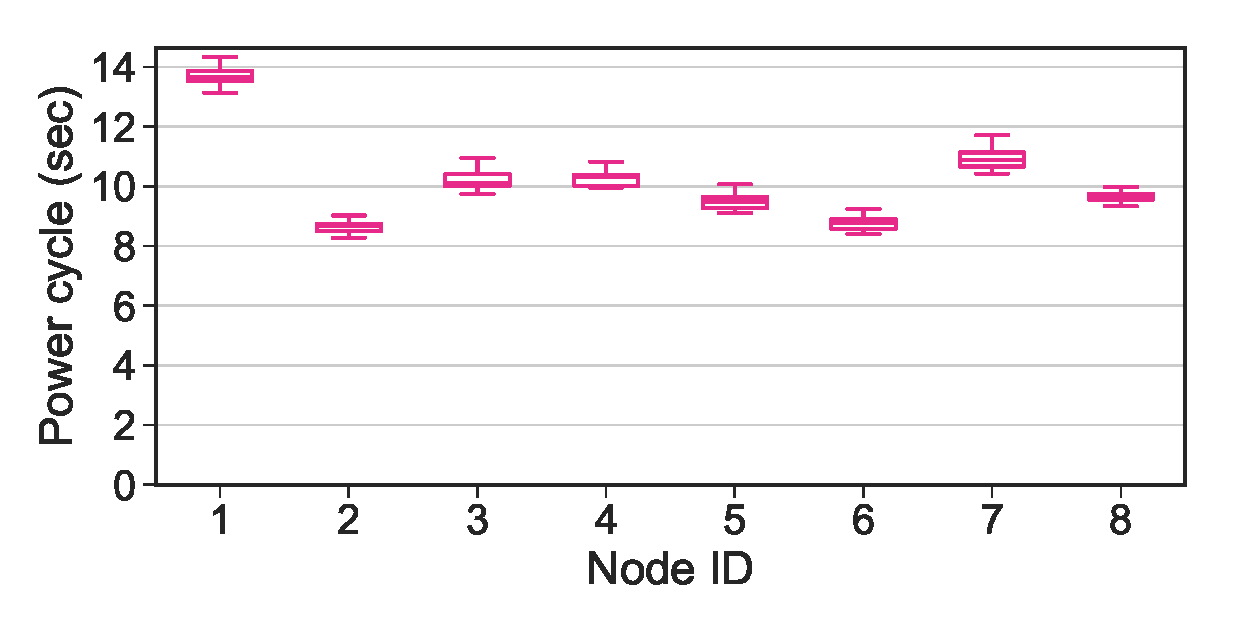
\includegraphics[width=\textwidth]{figures/light_power_cycles_len}
			\caption{Light}
		\end{subfigure}\hfill
		\begin{subfigure}{.49\columnwidth}
			\centering
			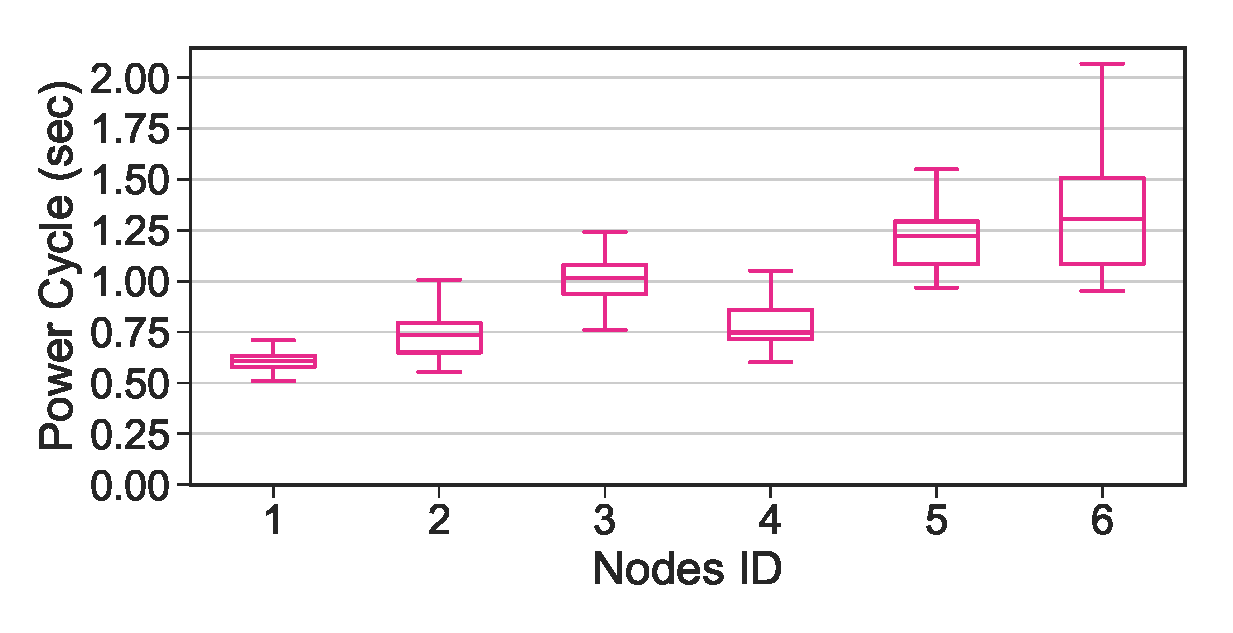
\includegraphics[width=\textwidth]{figures/rf_power_cycles_len}
			\caption{RF}
		\end{subfigure}\hfill
		\caption{nodes' power cycles length for different energy sources, and different energy buffer sizes.}
		\label{fig:power_cycles}
\end{figure} 


\subsubsection{Events classification}
\label{sec:event_classification}
Given the unique characteristics of \sys, it is important to classify the events, identifying the categories that \sys can monitor. Form \sys's perspective, we can classify the events into three categories:
\begin{itemize}
%
\item \textit{Short events}: are events that can be captured using single intermittent node. 
For example, a spoken word can be seen as a short event if the energy needed to recorded is less than what the energy buffer, i.e., the capacitor, of the intermittent sensor can store.
\item \textit{Long events}: are events that need more energy to be completely captured than what the energy buffer can store. Long events can be subdivided into two types: 
	\begin{itemize}
		\item \textit{complex}: is a long event and capturing part is insufficient to extract the embedded information.  For example, a spoken word can be seen as a long complex event if its recording requires more energy than what the energy buffer can store.

		\item \textit{simple} is a long event and capturing part of it is sufficient to extract the embedded information. For example, a rotating part of an engine that produce a particular sound. 
	\end{itemize}
\end{itemize}

\subsubsection{Effective Availability}
%
\todo{incomplete and needs to be rechecked}
%
Approaching continuous availability does not mean that \sys can successfully capture all events.
It can happen that an event is being only partially captured by one or more nodes, which may lead to unsuccessful event detection. Therefore, it is important to specify the probability of successfully capturing  events give particular \sys characteristics.  
%
First, let us start with a simple case, a \sys of a single node and a single event. 
Let us assume that a node has a power cycle has these characteristics ($t_\text{p}$, $t_\text{on}$). Thus, the percentage of the time the node is on is $\frac{t_\text{on}}{t_\text{p}}$.
Further, we do not assume any prior knowledge about the event arrival time.
Therefore, the probability of the event arriving at any moment in time is the same 
(mathematically, the event arrival time is a random variable drawn from uniform distribution).
Let us say the event is a short event (Section~\ref{sec:event_classification}) with a duration of $t_\text{e}$ unit of time, and it is given that it will happen in this power cycles
\footnote{Note that, an intermittent node's power cycle is repeating indefinitely; thus, when an event happens it will at least partially be within one  power cycle. We are focusing on this power cycle.}.
Consequently, we can compute the probability of successful event capturing as follows:

\todo{check the following equation}
\begin{equation}
	t_\text{s}(N) = t_\text{on}(N-1) + \frac{t_\text{off}(N-1)}{t_\text{off}(N-1)+t_\text{on}(N-1)} \times t_\text{on}(1) - t_\text{e},
		\label{eq:cisSenseModel}
\end{equation}

\subsubsection{Event-driven Sensing}
% \begin{figure}[t]
% 	\centering
% 		\begin{subfigure}{\columnwidth}
% 			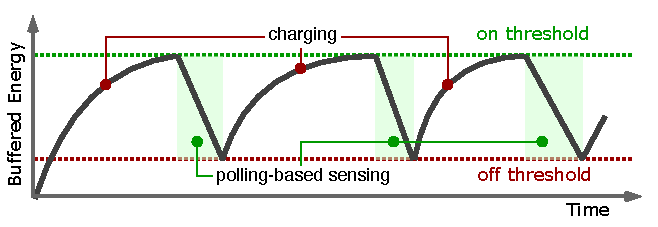
\includegraphics[width=\columnwidth]{figures/PowerCycleIntermittentSystem}
% 			\caption{When \sys does polling-based sensing, its energy consumption profile has, generally, two distinct rates: zero when it is charging, and a maximum when it is sensing.}
% 			\label{fig:pollingBasedSensing}
% 	\end{subfigure}
% 	\begin{subfigure}{\columnwidth}
% 		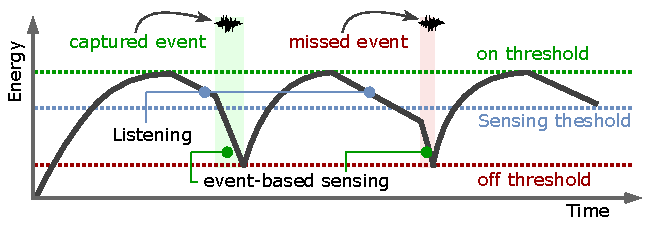
\includegraphics[width=\columnwidth]{figures/PowerCycleIntermittentSensor}
% 		\caption{When \sys does event-based sensing, it stays in low-power mode waiting for an external event to wake up the node. Consequently,  it has three distinct energy consumption rates: zero when it is charging, a maximum when it is sensing, and an in-between when it is sleeping. In favorable energy conditions, the sleeping mode may cause intermittent nodes to synchronize their power cycles on external events and miss the next ones.}
% 		\label{fig:eventBasedSensing}
% \end{subfigure}
% 		\caption{\fullsys (\sys) energy profile for different sensing strategies. Green bars highlight successful sensing operations  while the red bar shows a failed sensing attempt due to insufficient buffered energy.}
% 		\label{fig:cisPwrCycle}
% \end{figure} 
%
An intermittent sensor has a limited energy budget per power cycle. When it is tasked with a polling-based sensing activity, its energy consumption, generally, switches between two levels: zero when charging and maximum when it activates its microcontroller for data acquisition and processing. 
% see Figure~\ref{fig:pollingBasedSensing}. 
(Note that we assume that the microcontroller is the dominant energy consumer module of a node.) However, in event-based sensing, a node puts its microcontroller into low-power mode and waits (or listens) for an external event to wake up the microcontroller. For example, in our prototype, the command recognizer, we exploit the microphone's wake-on-sound feature to send an interrupt to the microcontroller, which will then start recording the sound samples from the microphone. 
%
%This hardware approach is most energy efficient, but can be mimicked in software by periodic polling (i.e.\ acquiring 1 sound sample and checking if it exceeds the acoustic noise floor). 
%
This wake-on-event style of operation is important as the minimal energy consumption during sleep significantly prolongs the period during which an event can be handled (for example, our prototype consumes 7 times less energy at sleep mode as compared to its active mode power consumption).
% , see Figure~\ref{fig:eventBasedSensing}.
This distinction between the energy consumption pattern of event-based and polling-based sensing will have an important consequence on how we model the probability of successful event capturing in these two different sensing strategy. 
% Although in reality the sleep and active phases draw quite different levels of power (128 vs. 849~$\mu$W on our hardware, see Table~\ref{tab:power_usage})
%
% we will model the life cycle of a sensor node simply as an on-period followed by an off-period (in which the node recharges its energy buffer) as that suffices to analyze the collective availability of a \sys.
%The idle listening mode, which is important for successful sensing, complicates the design of the \sys.


\subsection{Environment}


\subsubsection{Power States}
\label{sec:power_state}
A \sys can experience a wide range of ambient power intensities. For example, a solar-powered \sys may harvest no energy at night, modest energy from artificial light, and abundant energy from direct sunlight.  Generally, we can identify four different \sys powering states: 
\begin{itemize}
		\item \textit{Targeted power state}---These are the powering conditions that the \sys is designed for. In these  conditions, the \sys should work intermittently and have sufficiently randomized power cycles to uniformly distribute its intermittent nodes on-times and meet the desired availability percentage (Figure~\ref{fig:cisModel}). In general, the targeted powering conditions should be near worst energy harvesting conditions to ensure that the system is properly functioning for the majority of the time.
		\item \textit{Under-targeted power state}---Ultimately, the ambient energy is an uncontrollable power source, and it is not hard to imagine scenarios where a \sys will be under-powered or even comes to complete and long power down (for example, a solar \sys will come to a perpetual power down in the darkness). In general, for under-targeted energy conditions, the \sys behavior can be considered as undefined.
%
\begin{figure}
		\centering
		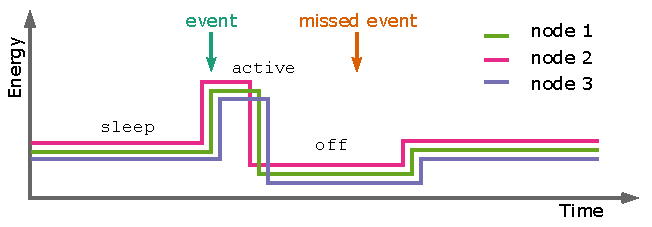
\includegraphics[width=\columnwidth]{figures/hibernating_power_state}
		\caption{\fullsys is in a hibernating power state when the energy harvesting rate approximates the energy consumption rate at the sleeping (or low-power) mode. In this state, the intermittent nodes lose the randomization in their power cycles. Thus, all the nodes capture the same event and power down shortly after missing the subsequent ones. Consequently, the \sys senses intermittently and does not take advantage of its redundant intermittent nodes to approach continuous sensing.}
		\label{fig:noRand}
\end{figure} 
%
		\item \label{it:hibernating} \textit{Hibernating power state}---In event-based sensing scenarios, the intermittent nodes of a \sys sleep in low-power mode waiting for an external event to wake them up. If the energy conditions are relatively higher than the targeted conditions, the nodes may not die and sustain their sleeping power consumption. This will cause them to synchronize their wake-ups on the first incoming event and their power down as the event capturing process depletes their energy buffers quickly. Consequently, the \sys may miss the next incoming events (specially if the events happens to arrive in bursts) causing it to sense intermittently instead of continuously, see Figure~\ref{fig:noRand}. 
		\item \label{it:continuous} \textit{Continuous power state}---Under direct mid-noon sun even a tiny solar panel can continuously power a sensor. In such conditions, the \sys will sense continuously without the need for randomization. Therefore, the job of a single node will be repeated $N$ times, and instead of sending a single message to a battery-powered or tethered sink---to push the data to the internet---$N$ identical messages will be sent which waste a lot of energy. 
				
\end{itemize}
%
% \begin{figure}
% 		\centering
% 		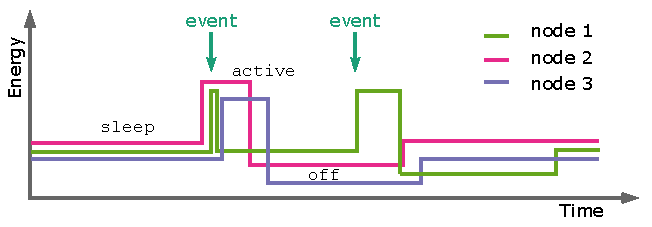
\includegraphics[width=\columnwidth]{figures/randomized_response}
% 		\caption{Randomized response helps in mitigating the hibernate-power-state problem. Also, it reduces the number of duplicated captured events when the \sys is overpowered. However, effective randomization strategy must be energy aware.}
% 		\label{fig:rand}
% \end{figure} 

The inefficiencies highlighted in the hibernating and continuous power states can be mitigated by enforcing randomization on the response of intermittent nodes 
% (Figure~\ref{fig:rand})
: when a node is woken up by an external event it responds to that event with a certain probability. However, if the randomized response is enforced all the time, then the \sys will have a lower probability of catching events during the targeted energy conditions. Therefore, the \sys has to distinguish between the targeted and above-targeted energy conditions and randomize its response only during the hibernating and continuous power states. 


Choosing a fix response probability is an inefficient way of dealing with the over-powering problem as the number of active intermittent nodes at a given moment is a function of the total number of intermittent nodes and the power intensity at that time. Therefore, efficient randomization requires intermittent nodes to estimate the number of active nodes at the moment of an external event arrival (which is discuss it next) and respond proportionally.


\subsubsection{Intermittent Timing}
\label{subsec:interTimer}
%
\begin{figure}[t]
		\centering
		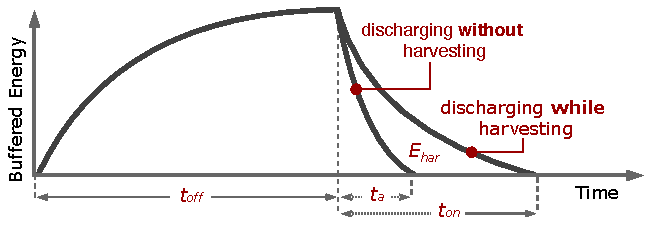
\includegraphics[width=\columnwidth]{figures/softwareClock}
		\caption{....}
		\label{fig:softwareClock}
\end{figure} 
%

Timing is a key building block of sensing systems. However, it is missing on intermittent nodes unless an additional dedicated timer circuit is added to them~\cite{hester2017timely}. Here we would like to propose an alternative way that does not require additional timer hardware. Obviously, the on-time of an intermittent node can be measured using the microcontroller's built-in timers. However, the difficulty is \textit{how an intermittent node can time its own off-time?}. Actually, answering this question does not only enable timing on intermittent devices but also enables them to estimate the richness of the ambient energy. 
%
\paragraph{Timing the death} 
Algorithm~\ref{algo:offTime} shows how a node can estimate its off-time. The basic idea is that a node measures its on-time while harvesting (Line~\ref{lin:ontime}) and compares it to the time required to drain the super capacitor without charging. The additional on-time $\Delta{t}$ is the result of the energy accumulated while executing. (Line~\ref{lin:deltat}). By assuming a relatively stable charging rate, a node can calculate how long it will be off charging (Line~\ref{lin:ehar}-\ref{lin:offtime}). Obviously, in order for the time estimation to be correct, the reference time and the on-time measurement must be done with same load ($a$). %\textcolor{red}{\bf Stephan: not sure what is meant here with "with same load"??/}
% off-time estimation 
\begin{algorithm}[t]
	\captionof{algorithm}{off-time estimation}
    \label{algo:offTime}
    \small
    \begin{algorithmic}[1]
		\State \Call{$f_\text{reboot}$}{$u$} $= u{+}{+}$ \Comment{power reboot counter}
		\State $i \leftarrow $ \Call{$f_\text{reboot}$}{$i$} \Comment{$i$ is a persistent variable}
		\State $E_\text{buf}$ \Comment{Size of energy buffer}
		\State $t_a$ \Comment{time of discharging $E_\text{buf}$ at load $a$, no harvesting}
		\State$ t_{i} \leftarrow x $ \Comment{timing every $x$ power cycles}
		%
		\If{$(i\mod t_{i})=0$}
		    \State $i=0$
			\State \Call{$f_\text{load}$}{$a$} \Comment{set node load to $a$ }
			\State \label{lin:ontime} $t_\text{on} \leftarrow$ \Call{$t_\text{pers}$}{\null} \Comment{persistent infinite loop}
		\EndIf
		\If{$i=0$}
			\State \label{lin:deltat}$\Delta{t} = t_\text{on}-t_a$  \Comment{time difference due to charging}
			\State \label{lin:ehar}$E_\text{har} \leftarrow (E_\text{buf}\div t_a)\times\Delta{t}$ \Comment{harvested energy}
			\State $P_\text{in} \leftarrow E_\text{har}\div{t_\text{on}}$ \Comment{incoming power}
			\State \label{lin:offtime}$t_\text{off} \leftarrow E_\text{buf}\div P_\text{in}$
		\EndIf
	\end{algorithmic}
\end{algorithm}

\subsubsection{Nodes overlapping}
\begin{figure}[t]
		\centering
		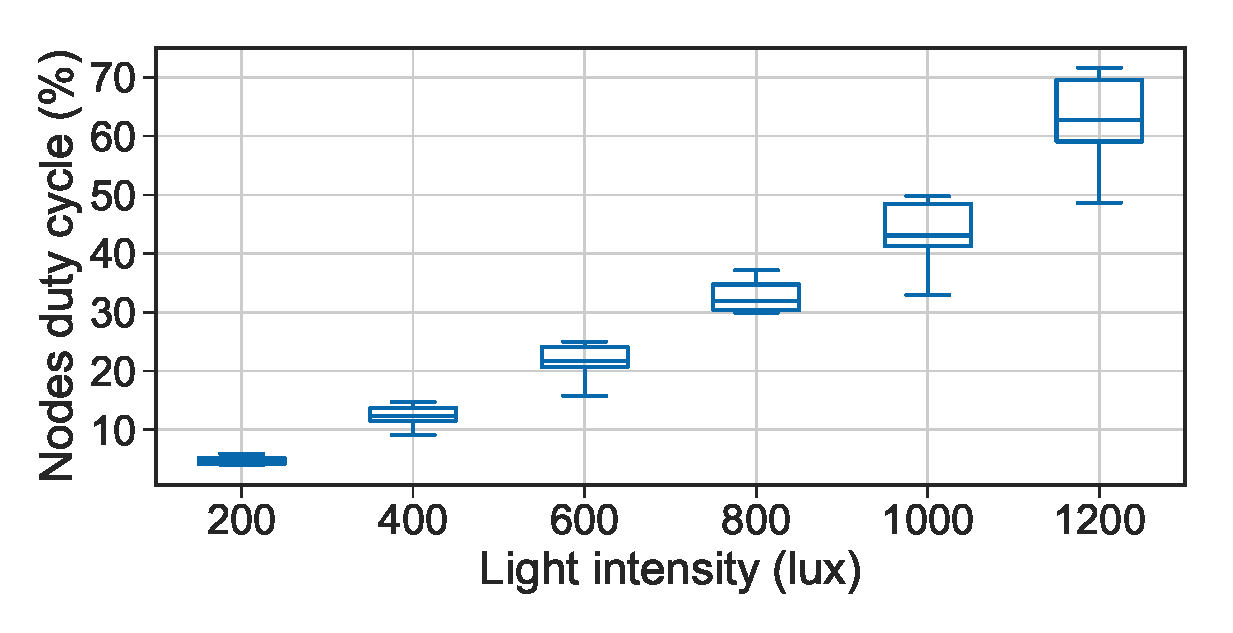
\includegraphics[width=\columnwidth]{figures/cis_dutyCycle.eps}
		\caption{The average duty cycles of eight intermittently powered nodes for different light intensity. In general, an individual node's duty cycle is a good indicator of the average duty cycle of its \sys.}
		\label{fig:cis_nodes_dutyCycle}
\end{figure} 

\begin{table}
		\centering
		\caption{Measuring intermittent nodes overlapping of a \sys of 8 intermittent nodes for different light intensities.}
		\begin{tabular}{lll}
				\hline
				light intensity (lux) & mean & std    \\
				\hline
				300	                  & 1.01 & 0.85   \\
				500                   & 1.63 & 0.98   \\
				800                   & 2.88 & 1.50   \\
				1200                  & 5.05 & 1.08   \\
				\hline
		\end{tabular}
		\label{tab:clusters}
\end{table}


In order for a node to estimate the number of active nodes at a given moment, first, it has to know the total number of nodes ($N$) in its \sys, which we assume to be known to the nodes before deployment. Second, this analysis is built on the observation that a node's on-time is a good indicator about the on-times of other nodes in the \sys, see Figure~\ref{fig:cis_nodes_dutyCycle}. A node can measure its on-time $t_\text{on}$ and off-time $t_\text{off}$ using  Algorithm~\ref{algo:offTime} (or an external dedicated timer~\cite{hester2017timely}). Then, it can estimate the maximum time span ($t_\text{max}$) of its \sys, which is the total duration of the nodes' on-times when they are aligned next to each other, as follows
\begin{equation}
t_\text{max} = N\times t_\text{on}.
		\label{eq:max_time}
\end{equation}
Then, from Equation~\ref{eq:cisModel}, the node calculates the \sys expected on-time ($t_\text{on}(N)$). As we argued in Section~\ref{subSec:availability}, nodes on-times are uniformly distributed over the \sys power cycle. Thus, the overlapping on-time is also uniformly distributed over the \sys on-time. Then, a node can calculate the average number of active intermittent nodes $n_\text{active}$ using the following formula,
\begin{equation}
	n_\text{active} = t_\text{max} \div t_\text{on}(N).
	\label{eq:active}
\end{equation}
and choose the proper randomization factor. If a second event, however, happens shortly after the first one, a node needs to update $N$ as follows, 
$$
N = N - n_\text{active}-1
$$
the $-1$ is because the node itself decided not to react on the first event. 

Table~\ref{tab:clusters} shows the average number of overlaps of an 8-nodes \sys for different light intensities. These measurements validate that nodes overlapping time is uniformly distributed over the \sys on-time. For example, at $\SI{1200}{lux}$ an individual node of our \sys has a duty cycle of $\approx$\,62\%. If we multiply it by the number of nodes (Equation~\ref{eq:max_time}) we get about 500\%. Figure~\ref{fig:cisModel} indicates that a \sys with eight nodes of duty cycles above 50\% has near 100\% availability. From equation~\ref{eq:active}, we find that the expected number of clustered nodes is 5 which is what Table~\ref{tab:clusters} also shows. 








































